The identification of rich wind resources have become important together with the increasing focus on green energy \cite{WindPowerGenerationUsingANN}. It is important to analyse and predict the wind power generation at a certain location before placing actual windmills. 
Wind speed, relative humidity and generation hours of the windmills are used as input for a Artificial Neural Network in \cite{WindPowerGenerationUsingANN}. It can come as no surprise that the meteorological factors like wind speed and air density have a huge impact on the wind power generation. Figure~\ref{fig:energyGeneration} shows how the monthly energy generation increases with the monthly average wind speed. 

\begin{figure}[h!]
\centering
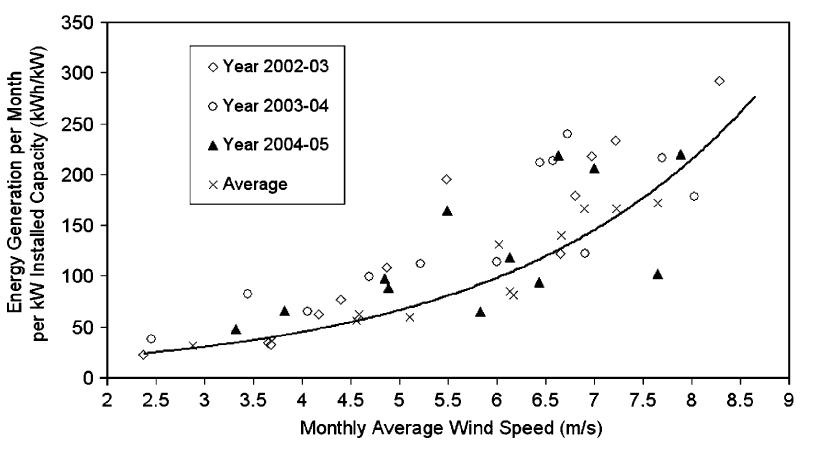
\includegraphics[width=0.8\linewidth,natwidth=898,natheight=587]{billeder/EnergyGenerationVsWindSpeed.png}
\caption{The influence of wind speed on the energy generation \cite{WindPowerGenerationUsingANN}}
\label{fig:energyGeneration}
\end{figure} 

The more "heavy" the air, the more energy is received by the windmill turbine. The humidity increases as as air density increases and because wind energy is proportional to air density the prediction algorithm needs humidity as input because it also accounts for temperature and pressure \cite{AirDensityInForecast}. Moist air is lighter than dry air because water molecules are less dense than the molecules in dry air such as oxygen and nitrogen. This basically means that the more air molecules like oxygen and nitrogen the more wind energy.

The last parameter in their prediction algorithm is generation hours which is the period in which the turbines produce power. The number of hours are influenced by f.x mechanical breakdowns, scheduled maintenance and low wind speeds. It is clear the the more generation hours the more energy is produced as seen in figure ~\ref{fig:energyGenerationFromHours}. The generation hours are hard to predict but can be calculated from past years up-time together with the expectations of the company delivering the windmills.  

\begin{figure}[h!]
\centering
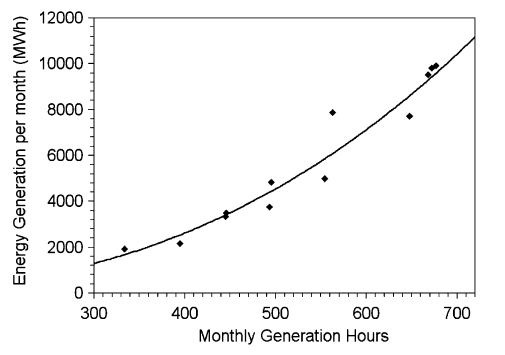
\includegraphics[width=0.8\linewidth,natwidth=898,natheight=587]{billeder/GenerationHourVSGeneration.png}
\caption{The influence of generation hours on energy production \cite{WindPowerGenerationUsingANN}}
\label{fig:energyGenerationFromHours}
\end{figure} 

The Artificial Neural Network trains 3-year dataset containing the mentioned input parameters. The input parameters are during the training compared to the output variable which is the wind energy output of the turbine. See figure~\ref{fig:annArchitecture} for the architecture.
\\[0.5cm]
\begin{figure}[h!]
\centering
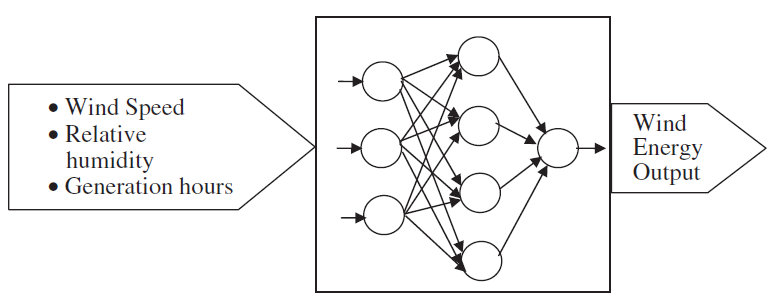
\includegraphics[width=0.7\linewidth,natwidth=898,natheight=587]{billeder/ANNwindSpeedPrediction.png}
\caption{Artificial Neural Network architecture from \cite{WindPowerGenerationUsingANN}}
\label{fig:annArchitecture}
\end{figure}

Another approach is seen in \cite{5} where the algorithm produces weighted nearest-neighbor (NN) tables to generate wind power curves based on available wind speed and direction from an online weather-data source. The weighted approach allows the algorithm to adapt to seasonal changes by weighting newest results highest, and the power curves makes it possible to use the algorithm on different wind farms. This prediction is used to schedule jobs in data centers which is described in the Applications subsection.

The vitality of the forecasts is seen when it comes to placement of wind farms. Before investing billions of dollars in a new wind farm it is of utmost importance to put it in the best possible location in relation to wind statistics, e.g. force of the wind and how often the winds change in power and direction at the position. In \cite{4} they use MCP to predict wind statistics based on large amount of geographical-, weather- and historical data so that the farms can be placed best possible. This knowledge can in some way be transferred to our specific purpose but because we are dealing with decision making in real time we cannot use as heavy algorithms that do calculations for several weeks and months before giving a result. We must deliver the most accurate estimate without delaying the trader's work.
There is also a big difference in using billions of dollars on windmills. The companies have to be 100 percent certain that they can produce energy where you put them. When doing decision support we only aid the trader in his daily work by giving him a real time estimate for the next hour or perhaps the next week - they still need to take the final decision based on their experience and knowledge. In addition, we can also assume that the wind mills are placed in a the best possible location where we only need to predict the energy production based on the current weather.